\documentclass{beamer}
\usepackage[spanish]{babel}
\usepackage{graphicx}
\usepackage{url}
\usetheme{Warsaw}
\title{Proyecto de Programación 1er Semestre}
\author{Dylan Ramsés Cabrera Morales}
\date{\today}
\begin{document}
\begin{frame}
\maketitle
\begin{center}
\small{Grupo:C-122}
\end{center}
\end{frame}
\begin{frame}
\frametitle{Introducción}
Moogle es una aplicación que se encarga de realizar una búsqueda en un conjunto de documentos
\begin{figure}[h]
\centering
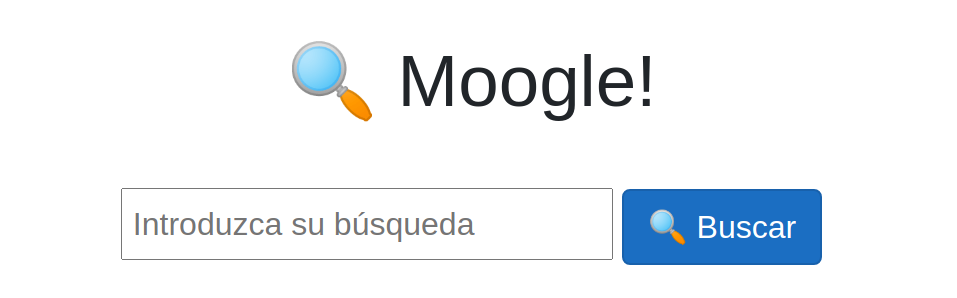
\includegraphics[width = 10cm]{moogle.png}
\caption{Moogle}
\label{fig:1}    
\end{figure}   
\end{frame}
\begin{frame}
\frametitle{Introducción}
Esta desarrollada con tecnología .NET Core 6.0. Se utilizó en esta Blazor como framework web
para la interfaz gráfica y el lenguaje $C\sharp$    
\end{frame}
\begin{frame}
\frametitle{Como funciona}
La aplicación se divide en dos componentes esenciales:
\begin{itemize}
    \item \underline{\textbf{MoogleServer}}: es el servidor web que se encarga de la interfaz gráfica
    \item \underline{\textbf{MoogleEngine}}: es la biblioteca de clases que se encarga de realizar la
    búsqueda
\end{itemize}
\end{frame}
\begin{frame}
\frametitle{Como funciona}
Para la lógica de este proyecto se siguieron una serie de pasos:
\begin{enumerate}
    \item Se procesa el texto de todos los documentos txt(se eliminan signos de puntuacion y procede
    a separar las palabras)
    \item Se calcula el TFIDF del corpus(Para más información sobre este algoritmo:\url{https://es.ryte.com/wiki/TF*IDF})
    \item Mediante la aplicación del modelo vectorial se calcula la magnitud de los documentos
    (Para mas información:\url{https://www.sciencedirect.com/topics/computer-science/vector-space-models})
\end{enumerate}
\end{frame}
\begin{frame}
    \frametitle{Como funciona}
    \begin{enumerate}
    \setcounter{enumi}{3}
        \item Se realizan todos los procedimientos mencionados anteriormente sobre la query
        \item Se emplea el modelo vectorial para calcular la similitud de cosenos de los
        documentos(Para mas información:\url{https://es.wikipedia.org/wiki/Similitud_coseno})
        \item Se devuelve por orden de mayor a menor los documentos con más relevancia con 
        respecto a la consulta introducida por el usuario
    \end{enumerate}
\end{frame}
\begin{frame}
    \frametitle{Como utilizarlo}
    Para ejecutar el proyecto se debe abrir un terminal en la carpeta del proyecto y ejecutar
    el comando make dev. Al ejecutar este comando saldrá en consola Cargando Documentos.Debemos
    esperar a que carguen los archivos y nos salga en consola Documentos Cargados y ya Moogle 
    estará listo para realizar su búsqueda(este proceso de cargar los documentos no debe tardar
    más de un minuto)
\end{frame}
\begin{frame}
        \frametitle{Como utilizarlo}
        Ya a la hora de realizar la búsqueda escribimos una query y presionamos el botón Buscar
        (En la query no deben ponerse operadores ya que estos no fueron implementados). Ya realizada
        la búsqueda si la query fue encontrada con éxito nos saldrán los documentos que más se 
        asemejan a esta con un fragmento de texto. En caso de que no se encuentre dicha query se 
        da una sugerencia de que palabra quiso decir el usuario
\end{frame}    
\end{document}